\section{Description of the hardware structure and functionality}
In the following section, the hardware parts and functions will be introduced and described. The following part consists of sensor selection, ADC, pic uno32 board \& motor-shield.

\section{Hardware diagram}
The micro-controller is connected to the motor-shield and the motor-shield is then powering both motor 1 and motor 2. The sensor-array is sending the data collected to the micro-controller which then sends it further to the bluetooth unit. The bluetooth unit then writes the data to the terminal. 

 \begin{figure}[!ht]
    	\centering    		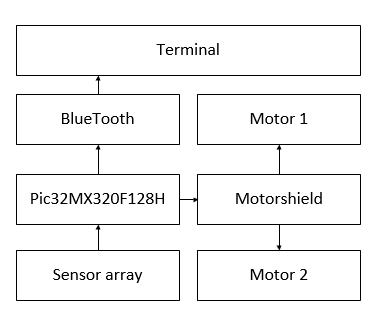
\includegraphics[width=.6\textwidth]{figures/hardwaredia2.png}
    	\caption{\text{Block diagram showing the hardware.}}
    	\label{Hardware diagram}
    \end{figure}

\section{Selection of sensor}

\begin{table}[htbp]
    \begin{tabular}{|l|l|l|l|}
        \hline
        Name                & QRE1113 board & OPB706A  & OPB704    \\ \hline
        Max sensor distance & 3mm                            & 1.27mm   & 3.8mm     \\ \hline
        Forward current     & 50mA                           & 20mA     & 40mA      \\ \hline
        Mounting            & On print                       & THT      & In casing \\ \hline
        Price               & 19.43DKK                       & 26.90DKK & 42.55DKK  \\ \hline
        Notes               & ~                              & ~        & ~         \\
        \hline
    \end{tabular}
    \caption{Table of a selection of sensors.}
\label{sensor_table}
\end{table}
The table is showing more sensors than the OPB 704, that is to show the price difference and the utility from sensor to sensor. \emph{(fig 2.1)}



\subsection{OPB704 Sensor}
The selected sensor for the line following robot will be the OPB704.\\
This sensor has been chosen from a range of criteria, most important being the optimal sensor distance and the easier mounting method. This method makes it more efficient to add several sensors in an array, which will be done with a 3D-printed mount. 

\sidebyimg{figures/opb704.jpg}{The sensor OPB 704}{figures/sensorarray.jpg}{3D printed sensor array module}


\section{Analog-to-digital converter (ADC)}

The purpose of the ADC is to convert the analog data from the sensors to digital data that can be managed by a computer - this allows data received from the blue-tooth transmitter on the product to be processed into readable data more easily, which is great for showing how the sensors are reacting. The sensors themselves cannot discern what they actually need to read, the sensors just read anything they can see and send that signal.

Analog signals can have a significant amount of noise - since any received noise is interpreted as part of the signal, a digital signal is not only more easy to work with, it will also provide more precise data. This will make for more accurate readings on the tachometer on the robot, which allows even more finely tuned monitoring of the robot and its working processes. \\

\subsubsection{ADC diagram} 
TBD? Er det relevant?

\subsubsection{This products usage of ADC}
Hvordan har vi gjort det i vores tilfælde?
<<<<<<< HEAD
TBD

\section{The Arduino Uno32 board}

Our main computing core is at the Arduino Uno32 board. The board was selected both because of previous experiences, and because it met the set requirements perfectly - most importantly it has twelve analog imputs to handle our array of seven sensors. This board utilizes the PIC32MX320F128 microcontroller, which features a 32-bit processing core running at 80Mhz with 128K of flash program memory and 16K SRAM data memory. This board allowed the most important aspects of the project to become reality; namely a GUI showing both the ADC readings as well as visualizing the sensor imputs, plenty of analog inputs to allow for the sensor array, and BlueTooth transmission of data from the robot unto a computer.\newline
The board is compatible for use with MPLAB IDE and the PICKit3 debugger.

\section{The motor shield - PKA03}

The motor shield was chosen because it is compatible with the Uno32 board, and fits perfectly within the scope of the project. It controls both motors and receives power from the 7.2 V lithium-ion battery pack mounted on the chassis itself. The motor shield is instrumental in providing motor controls to the product. To do this, it utilizes a specific electric circuit, called an H bridge.

\subsection{The H bridge}

An H bridge is a circuit that allows a voltage to be applied across a load in either direction. The purpose of this in the case of this project is to enable controls of the two motors in a way so that they can function individually, and both drive forwards and backwards.\\
At first, there were experiments with custom prints and a purpose-built h bridge on the first iteration of the motor shield. However after testing, it proved faulty and was changed to accommodate time constraints.
=======
TBD samarbejd med personen bag det
>>>>>>> origin/master
